% Computational Experiments for Evolutionary Pricing Games
\documentclass[a4paper,12pt]{article}  %% important: a4paper first
%
% \usepackage[notcite,notref]{showkeys}
\pdfoutput=1
\def\R{\textcolor{red}}
\usepackage{inconsolata}  % \tt font
\usepackage{natbib} 
\usepackage{amsthm}
\usepackage{newpxtext,newpxmath} 
\usepackage{microtype}
\linespread{1.10}        % Palatino needs more leading (space between lines)
\usepackage{xcolor}
\usepackage{pict2e} 
% \usepackage{bimatrixgame}
\usepackage{tikz} 
\usetikzlibrary{shapes}
\usetikzlibrary{arrows.meta}
\usepackage{amssymb}
%\usepackage{smallsec}
\usepackage{graphicx}
\graphicspath{ {./images/} {./PLOT/} }
%\usepackage[pdflatex]{hyperref}
\usepackage[hyphens]{url} 
\usepackage[colorlinks,linkcolor=purple,citecolor=blue]{hyperref}
%\usepackage{hyperref}
\urlstyle{sf}
\usepackage[format=hang,justification=justified,labelfont=bf,labelsep=quad]{caption} 
% \input macros-drawtree
\oddsidemargin=.46cm    % A4
\textwidth=15cm
\textheight=23.3cm
\topmargin=-1.3cm
\clubpenalty=10000
\widowpenalty=10000
\predisplaypenalty=1350
\sfcode`E=1000  % normal spacing if E followed by period, as in "EFCE."
\sfcode`P=1000  % normal spacing if P followed by period, as in "NP." 
\newdimen\einr
\einr1.7em
\newdimen\eeinr 
\eeinr 1.7\einr
\def\aabs#1{\par\hangafter=1\hangindent=\eeinr
    \noindent\hbox to\eeinr{\strut\hskip\einr#1\hfill}\ignorespaces}
\def\rmitem#1{\par\hangafter=1\hangindent=\einr
  \noindent\hbox to\einr{\ignorespaces#1\hfill}\ignorespaces} 
\newcommand\bullitem{\rmitem{\raise.17ex\hbox{\kern7pt\scriptsize$\bullet$}}} 
\def\subbull{\vskip-.8\parskip\aabs{\raise.2ex\hbox{\footnotesize$\circ$}}}
\let\sfield\mathcal
\newtheorem{theorem}{Theorem}
\newtheorem{corollary}[theorem]{Corollary}
\newtheorem{example}[theorem]{Example}
\newtheorem{lemma}[theorem]{Lemma}
\newtheorem{proposition}[theorem]{Proposition}
\theoremstyle{definition}
\newtheorem{remark}[theorem]{Remark}
\newtheorem{definition}[theorem]{Definition}
\def\reals{{\mathbb R}} 
\def\eps{\varepsilon}
\def\prob{\hbox{prob}}
\def\sign{\hbox{sign}}
\def\proof{\noindent{\em Proof.\enspace}}
\def\proofof#1{\noindent{\em Proof of #1.\enspace}}
\def\endproof{\hfill\strut\nobreak\hfill\tombstone\par\medbreak}
\def\tombstone{\hbox{\lower.4pt\vbox{\hrule\hbox{\vrule
  \kern7.6pt\vrule height7.6pt}\hrule}\kern.5pt}}
\def\eqalign#1{\,\vcenter{\openup.7ex\mathsurround=0pt
 \ialign{\strut\hfil$\displaystyle{##}$&$\displaystyle{{}##}$\hfil
 \crcr#1\crcr}}\,}
\def\zw#1\par{\vskip2ex{\textbf{#1}}\par\nobreak} 
\newdimen\pix  % bounding box height for eps files
\pix0.08ex
\newsavebox{\figA} 
\parindent0pt
\parskip1.3ex

\title{%
Computational Experiments for\\
Evolutionary Pricing Games
}

\author{
Bernhard von Stengel%
% \thanks{Department of Mathematics,
% London School of Economics, London WC2A 2AE, United Kingdom.
% Email:  b.von-stengel@lse.ac.uk}
}

\date{August 5, 2022
% \date{\today
% \\[1ex] --- draft, not for distribution ---
}

\begin{document}
\maketitle

\begin{abstract}
Here we describe computational experiments for
the project description
``Evolutionary Pricing Games'' (von Stengel, 2022), included
in this folder.
%
It is a documentation of the software, which at each stage
represents reproducable computational experiments.
%
It also outlines the next steps for more self-contained
runs (with fewer manual interventions)
of the experiments, and lists open questions. 
\end{abstract}

\section{What's new?}

\bullitem
This is the very first version of a documentation of the 
computational experiments, in an ad-hoc format (which will
evolve).
Subsequent versions may be more structured.

\bullitem
Implementation of a sophisticated ``guess your opponent''
strategy with interesting effects on the equilibria of the
tournament bimatrix game.

\bullitem
Some attempt at visualizing the bimatrix game payoff pairs. 

\def\dirname{{\tt 05Aug2022/}}
\def\equifile{{\tt equi11x5}}
\def\projfile{{\tt Evol-05Aug2022.pdf, Evol-05Aug2022.tex}}
\def\codepdf{{\tt 05Aug2022-play.pdf}}
\section{File inventory} 

{\einr 13em\parskip.3ex%
\rmitem{directory name:} \dirname 
\rmitem{main Python file:} {\tt play.py} ~ (run with python3)
\rmitem{code with line numbers:} \codepdf
% \rmitem{documentation:} {\tt comments}
\rmitem{output file:} {\tt output}
\rmitem{computed equilibria:} \equifile
\rmitem{plots folder:} {\tt ./PLOT}
\rmitem{project description:} \projfile
\rmitem{this file:} {\tt readme.pdf, readme.tex}
% \rmitem{graphics files:} {\tt }

}

\section{Description of the model and investigation}

The projection description \projfile\
describes a duopoly game investigated with the ``strategy
method'' by Keser (1992).

The present text describes and documents the computational
experiments to continue this research, by extending it
with
\bullitem
the implemention of some first pricing strategies
\bullitem
equilibrium analysis
\bullitem
evolutionary simulations (not yet implemented)
\bullitem
machine learning (not yet implemented).

\section{Purpose of this document and directory contents} 

The current directory \dirname, named by date, is meant to
contain a complete, self-contained snapshot of the project
at each stage.

It will be copied and updated with a new date at the next
iteration.

A more systematic solution might be to store it on github.
However, this requires technical knowledge of branch
management in git.
The current code is still small and copying seems fine for
now.

Its documentation in LaTeX is more important at the moment.

\R{Text parts in red} highlight points for improvement in
the current context, which may become kind of ``issues'' (as
in github) to become resolved in subsequent coding phases.
\R{Maybe they should be numbered here and later recorded as
``resolved''.}

\R{We can switch to Git, with the advantage that only
important files are stored in the repository and very easily
shared with {\tt git push} and {\tt git pull}, but have to
clearly mark those project snapshots, perhaps as
\textbf{releases}, that do work on their own.
We need tutorials on branch management.} 

\section{Current code capability} 

At present, the Python code {\tt play.py} contains
\bullitem
a number of duopoly pricing strategies as methods
\bullitem
a method {\tt match()} to match any two strategies against each other
\bullitem
a method {\tt tournament()} to match all low-cost strategies
of player 0 to all high-cost strategies of player 1, and
record the resulting payoffs to the two players in a
bimatrix game $(A,B)$.
This bimatrix game is then written to standard output to
find all its Nash equilibria via the program {\tt lrsnash},
currently by using the webpage {\tt
http://banach.lse.ac.uk}.
\R{Because {\tt lrsnash} exists as an executable C program,
starting it from Python should be automated next.}

\bullitem
The output of {\tt lrsnash}, via this manual route, is
stored in the equilibrium file \equifile.

% The file {\tt comments} explains the Python code in more
% detail with reference to its line numbers in \codepdf.
% This is not to clutter the Python file itself, \R{but the
% reference to line numbers is likely to outdate quickly.
% Maybe put these comments into the Python code after all?
% Using better documentation tools?}

\bullitem
The output of {\tt play.py} to standard terminal output {\tt stdout} is
recorded in the file {\tt output}.
Apart from $(A,B)$, it prints a sample run of two
strategies against each other, with the history of demand
potentials, prices, and profits of the two players,
and a descriptive list of the two players' strategies.

\bullitem
Graphical output:
In {\tt ./PLOT/}, a number of files are generated to 
display the payoff pairs in a suitable graphical format via
the Linux program {\tt gnuplot}.
\R{Improvement with Python packages seems appropriate.}

\subsection{Strategies}

In \projfile, Sections 4 and 5 describe some pricing
strategies.
They are implemented as Python methods.
Two minimum parameters of a strategy are player and time
period
\R{(player is always the first parameter; maybe the time
period should always be the second parameter for
consistency)},
and possibly additional parameters such as a price for the
first period.
All strategies have access to the past demand potentials and prices
of the players, but for the current time period can only
access the player's own demand potential.
Prices cannot be set below cost.

The following strategies are straightforward 
(because it is optimal, they always use the myopic monopoly
price in the last period):
\bullitem
the myopic monopoly price,
\bullitem
a constant price,
\bullitem
imitating the opponent's previous price.

A ``fightback'' strategy to reclaim a lost but aspired
demand potential turned out to be not so easy to implement
and has a first version {\tt fight}, and a more sophisticated
version {\tt guess}.

{\tt fight} is very aggressive because it never raises
prices back, which results in oscillations and a price war
when played against each other.

{\tt guess} remedies this, and has other features:

\bullitem
When the demand potential is favorable, it lets the firm's
price raise partially (weighted with a factor of 0.4
compared to the last own price with weight 0.6).
This allows convergence to cooperation near the monopoly
price (minus 7 for protection).
\R{It will be interesting if such a behavior, and these
weights and the parameter 7, which may not be optimal, is
learned in a neural net.}

\bullitem
Importantly, rather than reacting to the opponent's last
price, which seems to induce oscillating price wars, it
assumes that the determining variable for the opponent's
behavior is their \textit{sales number} (demand potential
minus price). 
It stores this as a static variable
(in Python: the global list {\tt oppsaleguess}) which is
updated with a multiplicative weight {\tt alpha} from last
time and then used to estimate the opponent price from their
\textit{current} demand potential $400-D$ (where $D$ is the
own demand potential) to reclaim the aspired potential in
the next round.

In order to test the imitation strategies and possible
responses against them, they are used for the column
player~1 against several constant strategies of the row
player~0.
In addition to the imitation strategies, 
each player's first strategy is the myopic strategy, and the
second strategy is the sophisticated {\tt guess} strategy.
Indeed, the latter two represent a (possibly fragile)
\textit{pure Nash equilibrium}, see below.
The size of $(A,B)$ is here $11\times 5$.

\subsection{Graphical output}

The generated bimatrix game $(A,B)$ contains payoff pairs
that reflect how the two players cooperate or compete for
any low-cost strategy (row) against high-cost strategy
(column).

We want to display the possible payoff pairs in the plane as
the possible ``region'' of cooperation versus competition,
and explore its Pareto frontier, where a gain of one player
can only be achieved at the expense of the other.

I try to display these payoff pairs not just as a collection
of dots but also in dependence on the player's strategies.
The following can be improved but is a start.

The directory {\tt ./PLOT} has to exist before {\tt play.py}
is run.
It will contain $m$ files for the $m$ strategies of
player~0, each with the pairs of payoffs in the respective
row of $(A,B)$.
These are then used with the program {\tt gnuplot}
(possibly \R{later to be replaced by Python plots}) to
display the payoff pairs.

The first two rows of $(A,B)$
are the myopic and the {\tt guess} strategy of player~0,
with the following payoffs:
% \\
% 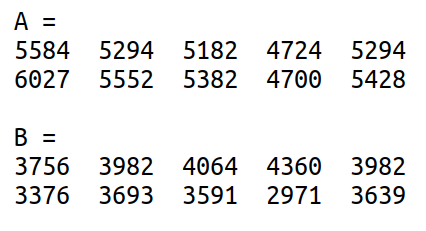
\includegraphics[width=7cm]{2rowsAB.png}
% \\
\begin{verbatim}
A = 5584  5294  5182  4724  5294    B = 3756  3982  4064  4360  3982 
    6027  5552  5382  4700  5428        3376  3693  3591  2971  3639 
\end{verbatim}
The five columns of $(A,B)$ are the strategies named
{\tt myopic, guess130, imit131, imit114.2, fight130}
of player~1, where 130, 131, 114.2, 130 are the starting
prices in the first period.
Against the myopic strategy of player~0, {\tt fight130}
performs the same as {\tt guess130} (with payoff pair
$5294,3982$).
Usually {\tt fight130} is much more aggressive and therefore
listed last.

The graphics show each payoff pair as a point in the plane
with the row player's payoff in the horizontal direction and
the column player's payoff in the vertical direction.
For each strategy of the row player (in the next picture
only for the first two rows), we connect these points by
four line segments for the five column strategies.
\\
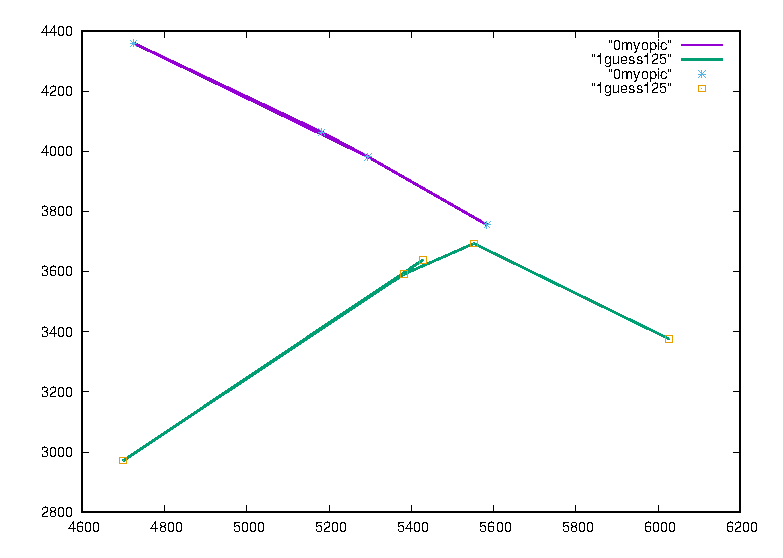
\includegraphics[width=15cm]{Pareto-manual.eps}
\\
This plot is generated (in directory {\tt ./Plot/})
with the Linux command 
\\
{\tt gnuplot gplot-manual} \
to produce the output file {\tt Pareto-manual.eps}.
The choice of colors and symbols is automatic.
The green line from right to left shows the performance of
{\tt guess125}, which is much better for the row player than
the myopic strategy.

For the 11 strategies of the full game, the symbols (like
the small yellow boxes above) are too
numerous, and only the lines are displayed, as follows:
\\
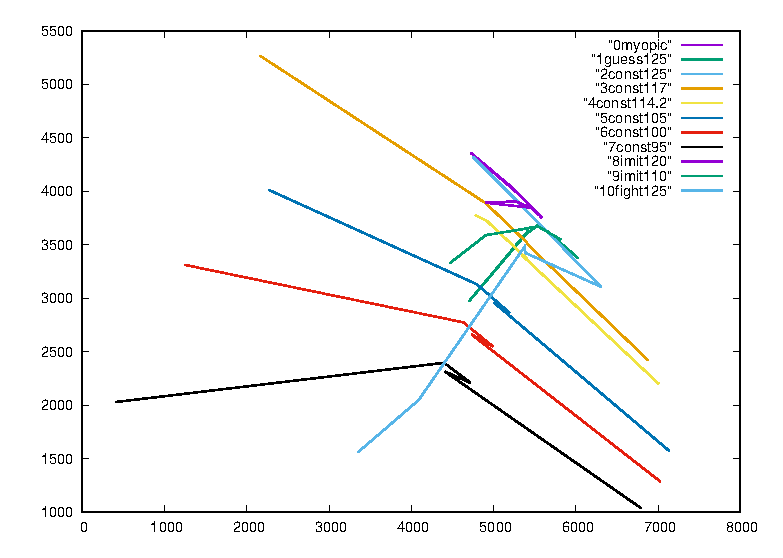
\includegraphics[width=15cm]{Pareto.eps}
\\
The lines, to be read from right to left, show the
following:
\bullitem
The right endpoint shows how each row performs against the
myopic strategy (first column) of the column player.
It can exploit that startegy, even with a constant price,
with marginal differences when that constant price is 
117, 114.2, or 105, and from then on even decreasing.
\bullitem
The second point of the first line segment (from the right)
shows the performance against {\tt guess130} of the column
player. It is ``retaliatory'' in that either both players
score low or both score high.
\bullitem
The left endpoint of each line shows how each row performs
against the last strategy {\tt fight130} of the column
player.
In fact, that strategy is able to exploit the constant-price
strategies of the row player of prices 100, 105, 117 shown
in red, blue, and dark yellow. 

Overall, there is already a wide spectrum of possible payoff
pairs and types of strategy.

\section{Equilibrium analysis}

This is most interesting. 
This game has already five mixed Nash equilibria.
However, three of these will have index $+1$ and two have
index $-1$.
Those with index $-1$ will not be dynamically stable.
\R{Having the index computation alongside would therefore be
a good idea.}

It turns out that for the column player, every strategy
except the myopic strategy (the first column) appears in a
mixed Nash equilibrium.
For the row player, there are four pure strategies that appear in
an equilibrium, which are
{\tt guess125,  const114.2, imit120, imit110}.

If the strategies that do not appear in a mixed equilibrium
are omitted, then the resulting $4\times4$ game
\textit{happens to have the same mixed Nash equilibria
(including a fully mixed one). This is not normally the
case: The omitted strategies may have suppressed some
equilibria that could appear in the smaller game.}
(Any mixed equilibrium of the larger game is also an
equilibrium of the smaller game, which has fewer
opportunities to deviate.)
Here, the five equilibria are as follows, in a manually
edited version of the output of {\tt lrsnash}.
\R{(This could be automated: reducing the display of
probabilities to 4 digits past the decimal point, and
suppressing pure strategies that have probability zero.)}

% All columns except the first ``myopic'' column appear 
\begin{verbatim}
    A = 5552  5382  4700  5428     B = 3693  3591  2971  3639
        5367  5383  4916  4776         3388  3387  3725  3779
        5458  5270  4900  5458         3847  3906  3895  3847
        5538  5318  4907  4467         3673  3642  3591  3328

    1  P1:  (1)  0.1134  0.2613  0.3468  0.2784  EP=  5201.93
       P2:  (1)  0.2400  0.3927  0.3266  0.0407  EP=  3661.12

    2  P1:  (2)  0.0501  0.1189  0.8310  0.0     EP=  5174.28
       P2:  (2)  0.0     0.5843  0.3116  0.1041  EP=  3828.49

    3  P1:  (3)  0.0     0.4705  0.5294  0.0     EP=  4912.79
       P2:  (3)  0.0     0.0     0.9771  0.0229  EP=  3815.0

    4  P1:  (4)  0.0     0.1957  0.0     0.8043  EP=  4938.55
       P2:  (4)  0.05    0.0     0.95    0.0     EP=  3617.22

    5  P1:  (5)  1.0     0.0     0.0     0.0     EP=  5552.0
       P2:  (5)  1.0     0.0     0.0     0.0     EP=  3693.0 
\end{verbatim}
The last row shows that {\tt(guess125, guess130)} is a
pure-strategy equilibrium.
Note, however, that the last row of the $4\times 4$ game
above has a payoff of 5538 which is not much lower than the
equilibrium payoff of 5552, so this pure equilibrium may be
fragile in the presence of other strategies.

\section{Plan of work}

The goal of this research is learning how to play well a
complex ``base game'', here the pricing game, which is too
complex to know in advance, against an unknown distribution
of opponents who themselves also evolve.

Here are some next steps.

\bullitem
\textbf{Remove the end effect.}
The pricing game runs over a fixed number of 25 periods,
which has an ``end effect'' that myopic play is optimal
in the last period (which could be extended with further
optimal equilibrium play in the preceding periods).
\R{It seems better to introduce a discount factor that
terminates the game with a fixed probability, say 4 percent
-- which should be a parameter -- after each round to
suppress this arbitrary end effect. \textit{In each match,
this will require multiple rounds because the number of 
rounds of interaction with the opponent is random.}
\textbf{It is probably also a good idea to start the random
generator with a fixed seed to make these random runs
reproducible, i.e. always giving the same payoff pairs.
Dependency on this seed should be tested separately.}}

\bullitem
\textbf{Introduce a learning model.}
In the pricing game, either Q-learning or some neural net
should be trained to determine the price for the next
period.

\bullitem
\textbf{Evaluate the performance of a strategy.}
The learning could be done, ad-hoc, in two phases:
\subbull
play against a fixed distribution of existing strategies.
The parameters of the learning model are adapted until it
plays well against an existing distribution of other
strategies.
\subbull
once learning has stabilized, the new strategy is entered
into the strategy pool.
\subbull
an evolutionary dynamics, such as the replicator
dynamics, is then run, which presumably changes the
distribution of strategies (one would need to recognize once
this has entered a certain orbit, perhaps via a
stabilization of the distribution of strategies).
\subbull
this new distribution is then used for the next
learning round.

\bullitem
\textbf{Alternative: no two phases of ``learning'' and
evolution.}
Alternatively, the learning could take place during the run
of the evolutionary dynamics. 
However, this may result in interaction effects that are
difficult to analyze.

\bullitem
\textbf{Dependency on the starting point.}
Evolutionary dynamics may result in different stationary
orbits or even equilibria depending on the starting
distribution.
For example, the pure equilibrium above may only be an
attractor in a small neighborhood of the equilibrium itself,
and otherwise lead to another equilibrium.

\bullitem
\textbf{Comparison of evolutionary dynamics and the tracing
procedure for equilibrium computation.}
The tracing procedure has a simple implementation via
Lemke's algorithm and leads to Nash equilibrium (of positive
index). 
It would be interesting to compare this, also dependent on
the starting point, with where evolutionary dynamics lead
to.
This comparison could already be tested for the $4\times 4$
game above.




\end{document}

